% Template for PLoS
% Version 1.0 January 2009

\documentclass[10pt]{article}

% amsmath package, useful for mathematical formulas
\usepackage{amsmath}
% amssymb package, useful for mathematical symbols
\usepackage{amssymb}

% graphicx package, useful for including eps and pdf graphics
% include graphics with the command \includegraphics
\usepackage{graphicx}

% cite package, to clean up citations in the main text. Do not remove.
\usepackage{cite}

\usepackage{color} 

% Use doublespacing - comment out for single spacing
%\usepackage{setspace} 
%\doublespacing


% Text layout
\topmargin 0.0cm
\oddsidemargin 0.5cm
\evensidemargin 0.5cm
\textwidth 16cm 
\textheight 21cm

% Bold the 'Figure #' in the caption and separate it with a period
% Captions will be left justified
\usepackage[labelfont=bf,labelsep=period,justification=raggedright]{caption}

% Use the PLoS provided bibtex style
\bibliographystyle{plos2009}

% Remove brackets from numbering in List of References
\makeatletter
\renewcommand{\@biblabel}[1]{\quad#1.}
\makeatother


% Leave date blank
\date{}

\pagestyle{myheadings}
%% ** EDIT HERE **


%% ** EDIT HERE **
%% PLEASE INCLUDE ALL MACROS BELOW

\newcommand{\Kcomment}[1]{{\color{blue}{[KJ: #1]}}}
\newcommand{\Acomment}[1]{{\color{red}{[AE: #1]}}}

\DeclareMathOperator{\Tr}{tr}
\newcommand{\mcond}{\,\middle\vert\,}
\newcommand{\cond}{\,\vert\,}
\newcommand{\loss}[1]{\mathcal L\left(#1\right)} 
\newcommand{\eloss}[1]{\mathcal L_0\left(#1\right)}
\newcommand{\T}{{\sf T}}
\newcommand{\E}[2][]{\mathbb E_{#1}\left[ #2\right]}    % expected value
\newcommand{\TODO}[1]{\emph{\small\color{blue}$\langle\langle$#1$\rangle\rangle$}}
\newcommand*\dif{\mathop{}\,d}
\DeclareMathOperator*{\argmin}{arg\,min}
\DeclareMathOperator{\rank}{rank}

%% END MACROS SECTION

\begin{document}
% Title must be 150 characters or less
\begin{flushleft}
{\Large
Improved estimation of neural correlations suggests detailed interactions in visual cortex
}
% Insert Author names, affiliations and corresponding author email.
\\
Dimitri Yatsenko,$^{1,\ast}$, 
Kre\v{s}imir Josi\'{c}$^{2}$,
Alexander S.~Ecker$^{1,3,4}$,
Emmanouil Froudarakis$^{1}$,
R.~James Cotton$^{1}$,
Andreas S.~Tolias$^{1,5}$
\\
\bf{1} Department of Neuroscience, Baylor College of Medicine, Houston, TX, USA
\\
\bf{2} Department of Mathematics and Department of Biology and Biochemistry, University of Houston, Houston, TX, USA
\\
\bf{3}  Werner Reichardt Center for Integrative Neuroscience and Institute for Theoretical Physics, University of T\"ubingen, Germany
\\
\bf{4} Bernstein Center for Computational Neuroscience, T\"ubingen, Germany
\\
\bf{5} Department of Computational and Applied Mathematics, Rice University, Houston, TX, USA

$\ast$ E-mail: yatsenko@cns.bcm.edu
\end{flushleft}

\section*{Abstract}
% Please keep the abstract between 250 and 300 words
Ambitious projects currently under way aim to record the activity of ever larger and denser subsets of neurons \emph{in vivo}.  Correlations measured in such recordings are anticipated to reveal important aspects of the functional organization of neural circuits.  However, estimation and interpretation of large correlation matrices from finite recordings are challenging.  Estimation can be improved by regularization: biasing of the estimate toward a low-dimensional, less variable approximation.  The amount of improvement depends on how parsimoniously the reduced approximation captures the dominant dependencies in the data.  Therefore, the selection of the most efficient estimator is an empirical question that informs about the types of dominant dependencies governing the system.

In this study, we sought the most statistically efficient estimator of neural correlations in recordings from large, dense groups of cortical neurons.  Using fast 3D random-access laser scanning microscopy of calcium signals, we recorded the activity of nearly every neuron in volumes of about 100 $\mu$m in diameter (150--350 cells) in mouse visual cortex.  We hypothesized that, in these dense recordings, the correlation matrix would be most efficiently represented by a sparse network of linear interactions between pairs of observed neurons combined with common latent factors representing unobserved inputs and global network fluctuations.  Indeed, in cross-validation tests, the covariance matrix estimator that imposed this correlation structure outperformed estimators regularized toward other plausible low-dimensional approximations. Furthermore, we found consistent relationships between the organization of sparse interactions inferred by this estimator and the physical distances and preferred orientation differences of pairs of cells.  Consistent with previous synaptic connectivity studies, the density of positive interactions decreased rapidly with distance and with difference in preferred orientation whereas negative interactions were less selective.  To further corroborate physiological interpretation of the inferred functional structure, future experiments will augment this analysis with measured synaptic connectivity, cell types, and brain states.


\section*{Author Summary}
% Please keep the Author Summary between 150 and 200 words
% Use first person. PLoS ONE authors please skip this step. 
% Author Summary not valid for PLoS ONE submissions.   
Correlations of the activity of neurons have proven useful as descriptors of the functional organization of neural circuits with implications for stimulus coding and circuit architecture.  Estimation of correlation matrices can be improved by imposing some kind of structure on the estimate with greatest improvement attained when the imposed structure efficiently captures real dependencies in the data. Using fast 3D two-photon imaging of calcium signals, we recorded the activity of large and dense groups of cells in mouse visual cortex and evaluated the cross-validated performance of correlation matrix estimators that imposed different kinds of structure. The correlation structure of the estimator that proved most efficient comprised a sparse network of partial correlations between pairs of neurons combined with several common latent factors, with both components required for efficient estimation. Because of its superior benefit for estimation, we proposed that this inferred structure could prove more relevant for the description of functional connectivity than the usual correlation matrix in densely sampled neural recordings. As a first application of this approach, we analyzed how the inferred connectivity related to distances between cells and differences in their preferred orientations and found basic agreement with previous studies of synaptic connectivity.

\section*{Introduction}
\subsection*{Neural correlations}
Pearson correlations between the spiking activity of pairs of neurons, or simply \emph{neural correlations}, are the most familiar descriptive statistics of neural population activity \cite{Averbeck:2006,Zohary:1994,Kohn:2005,Bair:2001,Ecker:2010}.  For example, \emph{noise correlations}, \emph{i.e.}~the correlations of stimulus response variability between pairs of neurons, have been shown to have profound theoretical implications for stimulus coding \cite{Zohary:1994,Abbott:1999,Sompolinsky:2001,Wilke:2002,Averbeck:2006,Josic:2009,Berens:2011,Ecker:2011}. In addition, neural correlations are hypothesized to reflect key features of functional connectivity in neural circuits.  Such interpretation is supported by a series of discoveries of nontrivial relationships between neural correlations and other aspects of circuit organization such as the physical distances between neurons \cite{Smith:2008,Denman:2013}, their synaptic connectivity \cite{Ko:2011},  stimulus response similarity \cite{Bair:2001,Kohn:2005,Cohen:2008,Cohen:2009,Ko:2011,Smith:2013b}, cortical layer specificity \cite{Hansen:2012,Smith:2013}, progressive changes in development and in learning \cite{Golshani:2009,Gu:2011}, changes due to sensory stimulation and global brain states \cite{Goard:2009,Kohn:2009,Ecker:2010,Renart:2010}, and others.

However, neural correlations do not submit to ready or unambiguous mechanistic interpretation.  Theoretical studies and simulations have shown that neural correlations on various temporal scales may arise from combinations of multiple mechanisms including  direct synaptic interactions, common inputs or correlated inputs, chains of multiple synaptic connections, oscillations, top-down modulation, and background network fluctuations \cite{Perkel:1967b,Moore:1970,Shadlen:1998,Salinas:2001,Ostojic:2009,Rosenbaum:2011}. 

\subsection*{Additional information in neural correlation matrices}
Yet, a complete correlation matrix provides more information than the equivalent number of isolated pairwise correlations. In early studies, the effects of correlations were extrapolated from isolated pairs to entire populations through simulation and theoretical analysis \cite{Shadlen:1998,Zohary:1994}. In contrast, modern multineuronal recordings from increasingly large and dense populations of highly interconnected neurons allow estimation of various low-dimensional representations of the entire correlation matrix, which can enable inquiry into the nature of underlying physiological mechanisms and computational principles.  

For example, one form of low-dimensional representation of the correlation matrix is its low-rank approximation. Low-rank approximations are particularly suitable for capturing shared fluctuations across the recorded population. Extracted through principal component or factor analysis, low-rank components of neural correlations have been analyzed in a number of studies with particular attention paid to their temporal dynamics \cite{Yu:2009}. 

Alternatively, the correlation matrix can be formulated through the partial correlations between pairs of neurons. The partial correlation between a pair of neurons is the linear correlation remaining after accounting for correlations to all the other neurons. Partial correlations carry particular significance when conditional dependencies between all the variables are thought to be dominated by linear effects. In such systems, zero  partial correlation between two variables implies their conditional independence.  Conditional independence between a pair of variables suggests a lack of direct interaction between the underlying processes. Therefore, estimation of networks of partial correlations (sometimes called \emph{association networks}) have been used to infer interactions between components in complex systems such as gene interaction networks \cite{Schafer:2005,Peng:2009} and functional connectivity between brain regions in fMRI signals \cite{Varoquaux:2012,Ryali:2012}. In \emph{elliptical distributions} (those of the form $x \sim \frac 1 Z g\left((x-\mu)^\T\Sigma^{-1}(x-\mu)\right)$, where $g$ is an arbitrary function, $Z$ is the scalar normalizer, $\Sigma$ is the covariance matrix) and the multivariate normal distribution in particular, interactions are completely defined by linear effects and partial interactions express conditional dependencies. A multivariate normal distribution specified through its graph of non-zero partial correlations is known as a Gaussian Graphical Model or Gauss-Markov Random Field \cite{Koller:2009}. With increasing departure from linearity, the correspondence between conditional dependence and partial correlations diminishes or completely breaks down \cite{Loh:2012}. For example, the coupling terms in pairwise Ising models have no direct relationship to the partial correlations \cite{Schneidman:2006,Tkacik:2006}.

\subsection*{Estimation of neural correlation matrices}
In this study, we pursued two related aims: (a)~improved estimation of neural correlation matrices and (b)~discovery of low-dimensional structure of correlations in recordings of multineuronal activity to facilitate their interpretation.  

The true correlation matrix is the normalized version of the true covariance matrix defined as
\begin{equation}\label{eq:true-covariance}
    \Sigma = \E{(x-\mu)(x-\mu)^\T},\quad \mu = \E{x}
\end{equation}
where $\E{\cdot}$ denotes expectation; $x$ is the $p\times 1$ vector of real-valued instantaneous firing rates in bins of duration $\Delta t$; and $\mu$ is the vector of mean firing rates.  The usual estimator of the covariance matrix is the \emph{sample covariance matrix} $C_{\sf 0}$ computed from the empirical sample of observations $x(t),\; t=n(1,\ldots,n)$ as
\begin{equation}
    C_{\sf 0} = \frac 1 \nu \sum\limits_{t=1}^n (x(t)-\bar x)(x(t)-\bar x)^\T,\quad \bar x= \frac 1 n \sum\limits_{t=1}^n x(t)
\end{equation}
where $\nu$ is the number of degrees of freedom per neuron in the sample ($\nu=n-1$ if observations are independent). In this study, we keep the sample mean $\bar x$ as the estimate of the true mean $\mu$, but seek a better estimate of the covariance matrix than $C_{\sf 0}$.

Given a covariance matrix estimate $C$ (not necessarily the sample covariance $C_{\sf 0}$), the correlation matrix $R$ is calculated by normalizing $C$ by its diagonal (variance estimates):
\begin{equation}
    R = \left(I\circ C\right)^{-\frac 1 2} C \left(I\circ C\right)^{-\frac 1 2}
\end{equation}
Similarly, the matrix of partial correlations $P$ is computed as the negative normalized version of the \emph{precision matrix} (inverse covariance matrix) $C^{-1}$:
\begin{equation}
    P = -\left(I\circ C^{-1}\right)^{-\frac 1 2} C^{-1} \left(I\circ C^{-1}\right)^{-\frac 1 2}
\end{equation}
Here $\circ$ denotes entrywise matrix product (Hadamard product) and $I$ is the $p\times p$ identity matrix. Clearly, off-diagonal zeros in the precision matrix correspond to zero partial correlations. 

Estimation of the covariance matrix from a large population presents a number of numerical challenges.  The amount of recorded data grows only linearly with the population size whereas the number of estimated coefficients increases quadratically.  This mismatch leads to increased opportunities for spurious correlations, to overestimation of shared activity (\emph{i.e.}\;overestimation of large eigenvalues) \cite{Ledoit:2004}, and to poorly conditioned estimates of the partial correlations \cite{Schafer:2005}.

Estimation can be improved through \emph{regularization}: the deliberate biasing of the estimate toward a low-dimensional approximation \cite{Schafer:2005,Bickel:2006}.  The usual estimate $C_{\sf 0}$ has the advantage of being unbiased ($\E{C_0}=\Sigma$) but, on average, it falls far from $\Sigma$ due to its sensitivity to sampling noise in training sample.  Low-dimensional estimates of various forms are typically less susceptible to sampling noise but are also liable to introduce their respective biases away from truth $\Sigma$.  Regularization works by striking a favorable balance between bias and variability. Regularization can produce \emph{some} improvement even with an arbitrary target estimate that has no relation to the true dependencies in the data.  Yet, when the target estimate is well suited for capturing the important features of the true covariance matrix with few terms, it will introduce minimal bias and outperform other estimators. 

To illustrate challenges of estimating the correlation matrix from a finite sample, we briefly consider a regularization scheme based on \emph{covariance selection} (Figure \ref{fig:01}) \cite{Dempster:1972}. In covariance selection, the estimate is produced by fitting only an optimal subset of the coefficients of the precision matrix while setting the rest to zero. We estimated the covariance matrix of a period of a somatic calcium signals of a group of 298 neurons in mouse visual cortex using both the sample covariance matrix (Fig.\;\ref{fig:01}\,A, B) and covariance selection (Fig.\;\ref{fig:01}\,C). Due to the low-pass filtration effect of calcium dye kinetics, correlations in unprocessed calcium signals are higher than typical firing rate correlations on shorter temporal scales. The apparent similarity of the two estimates belies the utterly different partial correlation structure (Fig.\;\ref{fig:01}\,D, E): the regularized estimate is produced from the same data by zeroing the optimal set of 31,501 (71.2\%) of the off-diagonal coefficients of the precision matrix and fitting the remainder. Estimation by covariance selection is attractive for several reasons: First, it has fewer free parameters and is therefore less susceptible to sampling noise, yielding estimates that are, on average, closer to truth $\Sigma$. Additionally, if we assume that partial correlations do indeed reflect elements of the functional connectivity in the circuit, the second estimate also appears more plausible: in neural circuits, each neuron only interacts with a fraction of the entire population.

\subsection*{Model selection}
However, covariance selection is but one of numerous possible low-dimensional approximations of the covariance matrix. Indeed any probabilistic model of the joint population activity regularized toward a small number of parameters automatically defines a low-dimensional approximation of the covariance matrix. Models that accurately reflect the dominant functional dependencies in the circuit, its so-called `functional connectivity', will tend to produce estimates that are nearest to the true value of the covariance matrix and are said to be more \emph{efficient} than the other estimators or to \emph{dominate} the other estimators. An estimator's superior efficiency can be ascertained by cross-validation.  Because different types of neural circuits are governed by different types of dependencies, different probabilistic models and covariance matrix estimators may dominate in each case. The estimator that is shown to dominate all others for a specific type of neural circuit may be proposed as the best descriptor of the low-dimensional representation of the correlation structure of the system of interest. Its structure may then be analyzed and related to the circuits anatomical organization.  

\subsection*{Summary of findings}
In this study, we compared four regularized covariance matrix estimators biased toward different respective low-dimensional correlation structures: `shrinkage toward diagonal' or $C_{\sf diag}$, `shrinkage toward a multifactor model' or $C_{\sf factor}$, `sparse partial correlations' or $C_{\sf sparse}$, and `sparse partial correlations with latent units' or $C_{\sf sparse+latent}$.  First, we demonstrated that, in simulations with known true low-dimensional correlation structures, regularized estimators with matching types of low-dimensional structure generally dominated over the other estimators. We then used cross-validation to determine the most efficient estimator for the population activity of dense groups of neurons in mouse primary visual cortex. We found that $C_{\sf sparse+latent}$ consistently dominated the other estimators.  Estimate produced by $C_{\sf sparse+latent}$ revealed networks of interactions that differed substantially from networks of strongest correlations and depended strongly on the physical distance separating pairs of cells and on the differences in their preferred orientations. 


\section*{Results}
% Results and Discussion can be combined.

\subsection*{Covariance estimation}
We considered four regularized estimators based on distinct families of low-dimensional target estimates: `independent', `latent factors', `sparse interactions', and `sparse+latent' (Fig.~\ref{fig:02}\;row 1).  

In the first regularized estimator $C_{\sf diag}$, the target estimate is the diagonal matrix $D$ containing on its diagonal estimates of the variances.
The regularized estimate is obtained by linear \emph{shrinkage} of the unbiased estimate $C_{\sf 0}$ toward $D$ controlled by the scalar \emph{shrinkage intensity} parameter $\lambda \in [0, 1]$:
\begin{equation}
C_{\sf diag} = (1-\lambda) C_{\sf 0} + \lambda D
\end{equation}
The diagonal target estimate expresses the idea of a lack of dependence (or of linear association) between the activity of observed neurons (Fig.~\ref{fig:02}\,A).  
If this assumption aptly describes recorded data, then strong shrinkage toward $D$ will add little bias while strongly reducing the variability of the estimate. Shrinkage allows for partial commitment to the low-dimensional representation.  

In the second regularized estimator $C_{\sf factor}$, the target estimate is the factor model $F =  L L^\T + \Psi$ with $d$ factors so that $L$ is the $p\times d$ matrix of \emph{factor loadings} and the diagonal matrix $\Psi$ contains the independent variances of each neuron.
Then the estimate is 
\begin{equation}
C_{\sf factor} = (1-\lambda) C_{\sf 0} + \lambda F
\end{equation}
This estimator has two hyperparameters: the number of factors $d$ and shrinkage intensity $\lambda$. The target estimate $F$ expresses the assumption that correlated fluctuations in the population activity are driven by a small number of latent factors that affect many cells while direct interactions between cells are insignificant (Fig.~\ref{fig:02}\,B).   

The third estimator $C_{\sf sparse}$ is based on the assumption that all correlations are the result of direct linear interactions between pairs of observed cells and that such interactions occur only between a fraction of such pairs (Fig.~\ref{fig:02}\,C).  This assumption is enforced by setting to zero an optimal subset of the off-diagonal elements of the precision matrix.  Therefore, $C_{\sf sparse}$ is biased toward the assumption that correlations arise due to linear interactions between pairs of recorded neurons (Fig.~\ref{fig:03}C). Then the estimator is 
\begin{equation}
C_{\sf sparse} = S^{-1}
\end{equation}
where $S$ is a sparse matrix with a large fraction of zeros in its off-diagonal elements. The estimate has one hyperparameter to regulate the sparsity (fraction of off-diagonal zeros) in $S$.

Finally, we consider the fourth estimator $C_{\sf sparse+latent}$, which provides for both common latent factors interacting with all recorded neurons and sparse interactions between the recorded neurons (Fig.~\ref{fig:02}\,D). This estimator has the form \cite{Chandrasekaran:2010,Ma:2013}:
\begin{equation}
C_{\sf sparse+latent} = (S - LL^\T)^{-1}
\end{equation}
where, as above, $S$ is a sparse matrix and $L$ is a $d\times p$ matrix of factor loadings. The estimator has two hyperparameters: the number of latent units $d$ and the sparsity of $S$.

\subsection*{Simulation}
To verify our approach and to illustrate the performance of the four regularized estimators, we constructed four model populations of size $p=50$~neurons each with correlation structures of the same type as the target estimates of the first (Fig.~\ref{fig:02} Row 2). Panel A2 contains a diagonal correlation matrix matching the target of $C_{\sf diag}$. Panel B2 is a factor model with 3 factors conforming to the family of target estimates of $C_{\sf factor}$. Panel B3 is a correlation matrix with sparse partial correlations (76\% off diagonal zeros in the precision matrix). Finally, Panel B4 is a correlation matrix whose inverse is composed the sum of a sparse matrix (82\% sparse) and a low-rank component (rank=1).
Row 3 contains sample correlation matrices calculated from samples of size $n=1000$ from a multivariate normal distributions with the respective correlation matrices from Row 2.

To evaluate the performance of a covariance matrix $C$, we define a real-valued \emph{loss function} $\loss{C,\Sigma}$ such that it attains its minimum when $C=\Sigma$.  The loss function quantifies the error of the estimate, \emph{i.e.}~the deviation of the estimate $C$ from truth $\Sigma$.

In this study, we adopted \emph{negative normal log-likelihood loss}\footnote{
The loss function $\loss{C,\Sigma}$ is related to the multivariate log-likelihood function $L(\Sigma|C_{\sf 0})$ as
\begin{equation*}
    L(\Sigma|C_{\sf 0}) = -\frac p 2 \ln(2\pi) -\frac p 2 \loss{\Sigma,C_{\sf 0}}
\end{equation*}
}
defined as
\begin{equation}\label{eq:loss}
    \loss{C,\Sigma} = \frac 1 p\left[\ln \det C + \Tr(C^{-1}\Sigma)\right]
\end{equation}

We normalized the loss function  by $\frac 1 p$ to make its value comparable across different population sizes. 

This choice is motivated by mathematical convenience. Other popular choices for the loss function are the Frobenius norm of the difference $\|C-\Sigma\|_F$ \cite{Ledoit:2004,Schafer:2005}, Stein's entropy loss, and quadratic loss \cite{James:1961,Fan:2008}.  We expect that the main conclusions of our study will not change qualitatively under other well behaved loss functions.

To make the loss function to assume zero at its minimum when $C=\Sigma$, we define \emph{excess loss} as
\begin{equation}\label{eq:excess-loss}
    \eloss{C,\Sigma} = \loss{C,\Sigma}-\loss{\Sigma,\Sigma}
\end{equation}

In Figure \ref{fig:02}, row 4 shows the mean excess losses and their standard errors calculated from 30 samples of sizes n=250, 500, 1000, 2000, and 4000 for each estimator and each kind of ground truth. For each estimator, its hyperparameters were estimated by nested cross-validation (See Methods for more details.)

As expected, estimators with matching low-dimensional structures typically outperformed the other estimators. There were two exceptions to this observation. For small sample sizes, before the data were sufficient to reveal the true correlation structure and to  allow the correct model to dominate, estimates with simpler targets often outperformed the matching estimator.

When ground truth $\Sigma$ is not accessible, loss can be estimated solely from the data through \emph{validation}.  In validation, an additional independent \emph{testing sample} is used to compute an independent sample covariance estimate $C_{\sf 0}^\prime$.  Then \emph{validation loss} $\loss{C,C_{\sf 0}^\prime}$ can be used as an unbiased estimate\footnote
{
    Validation loss $\loss{C,C_{\sf 0}^\prime}$ is an unbiased estimate of loss $\loss{C,\Sigma}$ when $\loss{\cdot,\cdot}$ is \emph{additive} in its second argument so that 
 \begin{equation*}\label{eq:additivity}
 \loss{C,z_1} + \loss{C,z_2} \equiv \loss{C,z_1+z_2}
 \end{equation*}

Then the absence of bias can be shown:
\begin{equation*}
    \E{\loss{C,C_{\sf 0}^\prime}}=\loss{C,\E{C_{\sf 0}^\prime}}=\loss{C,\Sigma}
\end{equation*}

This property does not hold for some other popular losses such as Stein's entropy loss, for example, which prevents their substitution with corresponding validation losses. However, various other losses do conform to this constraints and could be used in this study.
} 
of loss $\loss{C,\Sigma}$.  Thus, estimators resulting in consistently lower validation loss can be inferred to produce estimates that are closer to truth than estimators with higher validation loss. 

With empirical data, acquiring a separate testing sample is not practical. Instead, $K$-fold cross-validation is used.  In cross-validation, the sample is divided into $K$ subsets of approximately equal size. In all computations in this paper $K=10$ was used.  Then each  subset is used as the validation sample with the other $K-1$ serving as the training dataset. The validation losses from each of such `folds' are averaged to produce \emph{cross-validation loss} or \emph{CV-loss} for short.  Let $C_{\sf 0}^{\{k\}}$ denote the sample covariance matrix computed from the $k^{th}$ subset and $C^{\{\setminus k\}}$ denote the results of  estimator $C$ trained on the remaining $K-1$ subsets. Then cross-validation loss for estimator $C$ is
\begin{equation}\label{eq:cv-loss}
    \ell_C=\frac 1 K \sum\limits_{k=1}^K \loss{C^{\{\setminus k\}},C_{\sf 0}^{\{k\}}}
\end{equation}
In the present formulation, $\ell_C$ is known as the cross-validated Gaussian log-likelihood (up to a constant offset and multiplier).

Since we only need to compare estimators against each other, we are only interested in \emph{relative} CV-loss of estimator $C$ with respect to reference estimator $C_{\sf ref}$:
\begin{equation}\label{eq:rel-cv-loss}
    \ell_{C,C_{\sf ref}} = \frac 1 K \sum\limits_{k=1}^K \left[
        \loss{C^{\{\setminus k\}},C_{\sf 0}^{\{k\}}} -
    \loss{C_{\sf ref}^{\{\setminus k\}},C_{\sf 0}^{\{k\}}} 
\right]
\end{equation}

In simulation, CV-loss accurately reproduced the differences between the estimators' excess losses, although with greater variability (Figure \ref{fig:02}, Row 5). For each kind of ground truth (Row 2), relative CV-losses were computed with respect to the estimator whose regularization target matched the structure of the respective ground truth: $\ell_{C,C_{\sf diag}}$, $\ell_{C,C_{\sf factor}}$, $\ell_{C,C_{\sf sparse}}$, and $\ell_{C,C_{\sf sparse+latent}}$. Just as with excess loss in Row 4, the means and their standard errors were computed from 30 samples  taken for each ground truth and for each sample size.

These simulation results demonstrated that, with sufficiently large sample sizes, the selection of the most efficient of several regularized estimators could be used to infer the type of low-dimensional structure present in the data, at least when one of the regularized estimators could capture such structure.

\subsection*{Covariance estimation in neural data}

We recorded the calcium activity of dense populations of neurons in the supragranular layers in primary visual cortex of anesthetized mice using fast random-access 3D scanning two-photon microscopy \cite{Reddy:2005,Katona:2012,Cotton:2013}. We presented 300 repetitions of full-field drifting gratings with two directions of motion or 150 repetitions with five directions (Fig.~\ref{fig:03}\,A) on one side of the visual field of anesthetized mice. Groups of cells loaded with a calcium-sensitive fluorescent dye were imaged and localized in 3D space (Fig.~\ref{fig:03}\,B and E) in the visual cortex on the contralateral side to the stimulus. With acousto-optic modulator (AOD) 3D steering of the laser, the located cells were imaged at high sampling rates with concurrent motion detection.  This technique allowed fast sampling (100--150 Hz) from large numbers (150--350) of cells in a small volume of cortical tissue ($200\times200\times100$ $\mu$m$^3$) in layers 2/3 and 4 (Fig.~\ref{fig:03}\,C). After downsampling the signal to 20 Hz, relative firing rates were inferred using sparse nonnegative deconvolution \cite{Vogelstein:2010} (Fig.~\ref{fig:03}\,C and D). Only cells that produced detectable calcium activity were included in the analysis. The average stimulus response was subtracted from each trial; the remaining signals were further downsampled into 150 ms bins to compute the noise correlation matrix (Fig.~\ref{fig:03}\,F and G). The durations of recordings dedicated to estimating the noise correlations ranged between 15--20 minutes.  Besides the high-repetition stimulus protocol for noise correlations, an orientation tuning stimulus protocol was used to map the orientation tuning of each cells (Fig.~\ref{fig:03}\,E). Overall, 31 imaged sites from 24 animals were included in the study.

In these highly localized populations both direct interactions between cells and common diffuse inputs are likely to contribute to the overall population variability, leading us to hypothesize that regularized estimates capable of accommodating partial correlations between specific pairs of cells (\emph{e.g.}\;$C_{\sf sparse}$ and $C_{\sf sparse+latent}$) would be more efficient than others. At the same time, average correlations were relatively small (Fig.~\ref{fig:03}\,G), to the advantage of estimates biased toward independence (\emph{e.g.}\;$C_{\sf diag}$). Finally, there is the possibility that the correlations structure is best explained by common fluctuations across the entire population, to the advantage of estimates biased toward low-rank correlation structure (\emph{e.g.}\;$C_{\sf factor}$, $C_{\sf factor+lowrank}$).

We found that estimator $C_{\sf sparse+latent}$ was more efficient than the other estimators (Fig.~\ref{fig:04}). The median relative CV-validation loss (Eq.~\ref{eq:rel-cv-loss}) of each of the estimates $C_{\sf 0}$, $C_{\sf diag}$, $C_{\sf factor}$, and $C_{\sf sparse}$ with respect to $C_{\sf sparse+latent}$ was significantly above zero ($p<0.001$, Wilcoxon signed rank test, for each).

\subsection*{Relationship of correlation structure to circuit architecture}
Having demonstrated that $C_{\sf sparse+latent}$ dominated the other estimators, we examined the elements of the low-dimensional structure revealed by this estimator for individual imaged sites. By its design, the sparse+latent estimator finds the optimal balance between a sparse network of partial correlations and shared common latent units. If this estimate dominates all other estimators evaluated thus far, it seems reasonable to hypothesize that these interaction may reflect underlying physiological interactions more closely than the usual correlations. In particular, the sparse component of the partial correlation matrix suggests direct interactions between pairs of neurons, whereas the low-rank component suggest common fluctuations such as those caused by common inputs or other collective synchronized activity. 

We examined the structure of the sparse+latent estimate in individual sites such as the example site first depicted in Fig.\;\ref{fig:03}. In this site, as in others, the regularized estimate of the correlation matrix appeared very similar to the unregularized sample correlation matrix (Fig.~\ref{fig:05}\,A and D). However, the corresponding partial correlation matrices differed dramatically (Fig.~\ref{fig:05}\,B and E). The partial correlation was decomposed into the sparse and low-rank components (Fig.\,\ref{fig:05}\,C). Although correlations were mostly positive, the sparse partial correlations (or `interactions'), although mostly positive, had a much larger proportion of negative values. The sparse component had 82.1\% sparsity (or 17.9\% connectivity), which corresponded to the average node degree (interactions per cell) of 52.5 (Fig.\;\ref{fig:05}\,G). The low-rank component was of rank 17.

In previous studies of the structure of correlations, a sparse network was produced by thresholding the correlations coefficients  above some level deemed significant and examining the network of correlations above that threshold \cite{Golshani:2009,Malmersjo:2013}. There was fairly little overlap between the network of interactions revealed by this thresholding method and those revealed by the sparse+latent estimator (Fig.\;\ref{fig:05}\,F). When thresholded to the same sparsity (82.1\%), only 42\% of cell pairs connected in one network were connected in the other while the average magnitude of such correlations was much lower in the case of the regularized estimator (Fig.\;\ref{fig:05}\,F, H, and I). In particular, many low sample correlations translated into negative interactions in the regularized estimate. Indeed, the absence of a correlation between pairs of cells that both correlate similarly to several of their neighbors should be considered as significant as a high correlation coefficient. Regularized partial correlations reveal such phenomena whereas regular sample correlations cannot.

The average partial correlations  revealed by the regularized estimator in all 31 sites were about 5 times lower than the sample correlations and  less variable across sites (Fig.\;\ref{fig:06}\,A). The average node degree of the sparse component of the partial correlations and the number of  inferred latent units varied widely between sites but generally increased with the recorded population size (Fig.\;\ref{fig:06}\,B and C). However, there was an inverse relationship between the number of latent units and the average node degree (Fig.\;\ref{fig:06}\,D). Several sites, even with relatively large population sizes, had fairly few pairwise interactions and were dominated by latent units.  These differences have multiple explanations, including differences in brain states and recording quality (neuropil contamination, motion). 

We also examined the relationship of differences in orientation preference and physical distances (lateral and by depth) between pairs of cells  to the average sample correlations, average regularized partial correlations, and inferred connectivity between them (Fig.\;\ref{fig:07}). The average partial correlations fell more rapidly with with difference in preferred orientation (Fig.\;\ref{fig:07}\,A and D) and lateral displacements at equal depths ($\pm 25\mu$m) (Fig.\;\ref{fig:07}\,B and E), and differences in depth at small ($\pm 25\mu$m) lateral displacements (Fig.\;\ref{fig:07}\,B and E).

The connectivity of partial correlations in the regularized estimate had different organization for positive and negative interactions. Positive interactions fell rapidly as a function of difference in preferred orientation (Fig.\;\ref{fig:07}\,G and J), lateral displacements (Fig.\;\ref{fig:07}\,H and K), and displacement in depth (Fig.\;\ref{fig:07}\,I and L). Negative interactions were much less selective (Fig.\;\ref{fig:07}\,G--L).


\section*{Discussion}
\subsection*{Functional connectivity from big neural data}
Transformational breakthroughs in neuroscience are anticipated to follow technological advances that will allow simultaneous recordings of the spiking activity of much larger subsets of neurons in functioning neural circuits than have been possible thus far. It far from certain whether massively multineuronal recordings will readily reveal new principles of neural function by application of current statistical techniques. Most common analyses of the functional connectivity rely on analyzing pairwise correlation coefficients, t-tests, ANCOVA, principal component analysis of correlated activity, and cross-correlations.  Traditionally, functional connectivity between regions has been defined as the level of correlation or synchronization between regions or cells. Without targeted stimulation and intracellular signals, synaptic connectivity could be inferred with some degree of confidence from the presence of sharp peaks or troughs in the cross-correlograms at offsets corresponding to typical synaptic transmission delays. However, even such effects can be explained by multiple effects besides monosynaptic connections while some strong synaptic connections do not necessarily produce a clear spike in the cross-correlogram. The situations is a bit more complicated in recording modalities, such as calcium imaging, in which only firing rates at lower temporal resolutions can be inferred and cross-correlograms with millisecond precision cannot be obtained. Therefore, some researchers have resorted to using simple correlations as proxies of functional connectivity. Yet, correlations are the end product of multiple cell interactions and, which do not always correspond to 


\subsection*{Comparison with other uses of neural correlations}
\subsection*{Meaning of interactions}
\subsection*{Fitting probabilistic models (\emph{e.g.}\;GLMs) vs.\;covariance estimation.}
\subsection*{Future directions}

\section*{Methods}
% You may title this section "Methods" or "Models". 
% "Models" is not a valid title for PLoS ONE authors. However, PLoS ONE
% authors may use "Analysis" 
\subsection*{Data Acquisition}
Fast 3D two-photon imaging of calcium signals \emph{in vivo} was performed as described in \cite{Cotton:2013}
\subsection*{Covariance Estimation}
TODO
\subsection*{Cross-validation}
TODO
\subsection*{Simulation}
TODO

\section*{Acknowledgments}
Genevera Allen

Eftychios Pnevmatikakis 

% The bibtex filename
\bibliography{references.bib}


\section*{Figure Legends}

\begin{figure}[!ht]
    \begin{center}
        %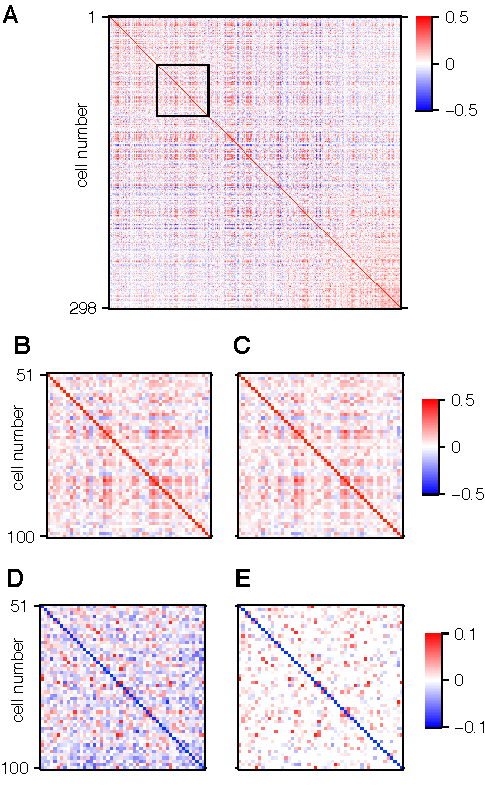
\includegraphics[width=8.3cm]{./figures/Figure01.pdf}
    \end{center}
    \caption{{\bf Illustration of regularized estimation of partial correlations.}
        {\bf A}. The sample correlation matrix of unprocessed somatic calcium signals from a population of cells in mouse visual cortex.
        The outlined square fragment is magnified in {\bf B}.
        {\bf C}. The same fragment of another estimate of the correlation matrix regularized to yield sparse partial correlations.
        Corresponding fragments of partial correlations matrices of the unregularized and regularized estimated are shown in {\bf D} and {\bf E}, respectively.
    }
    \label{fig:01}
\end{figure}

\begin{figure}[!ht]
    \begin{center}
        %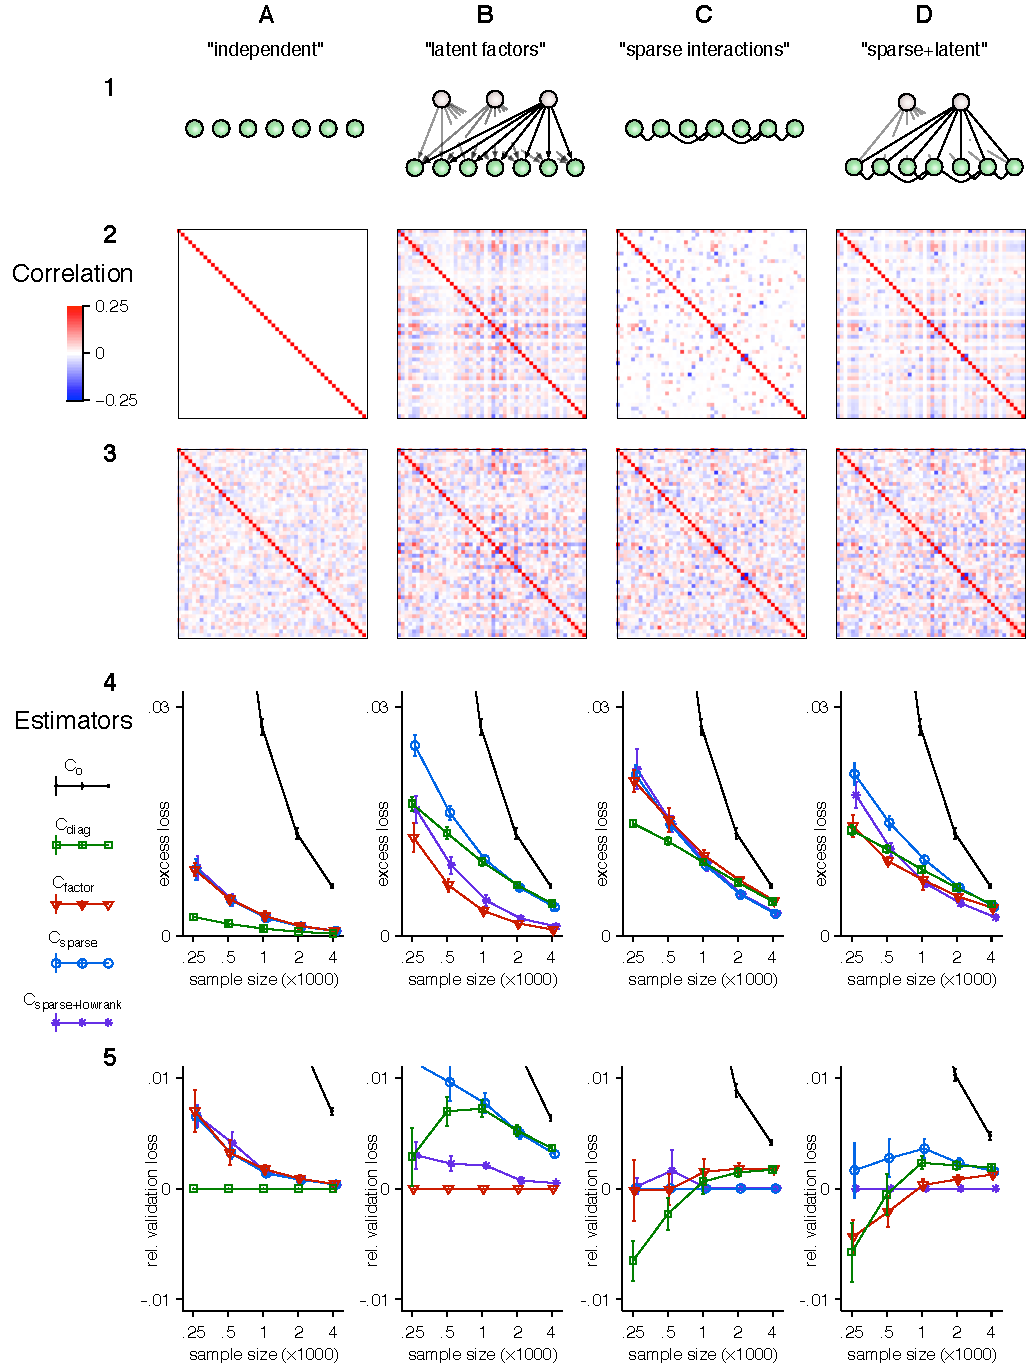
\includegraphics[width=17.35cm]{Figure02.pdf}
    \end{center}
    \caption{{\bf Estimators whose low-dimensional regularization targets can represent the structure of the true covariance matrix outperform other estimators.}
        {\bf Row 1.} Graphical representations of four types of low-dimensional structures of interactions between observed neurons (green spheres) and latent units (light-shaded spheres).
        In the `independent model' ({\bf A}), observed neurons exert no linear effects on one another neither directly nor through interactions with common latent units. 
        In `latent factors' ({\bf B}), the correlated activity of observed cells is driven by several latent units. 
        In `sparse interactions' ({\bf C}), the correlation matrix is defined by a set of linear interactions between observed neurons. 
        In `sparse+latent' ({\bf D}), correlations arise through direct linear interactions between some pairs of observed neurons and through interactions with common latent units. 
        {\bf Row 2.} Examples of $50\times 50$ correlation matrices corresponding to each type of low-dimensional structure. 
        The factor model ({\bf B}) has three latent units. 
        The partial correlation matrix of the sparse model ({\bf C}) is 73\% sparse.
        The `sparse+latent' matrix has one latent unit and its direct interactions are 78\% sparse.
        {\bf Row 3.} Examples of sample correlation matrices calculated from samples of 1000 observations taken from simulated random processes with corresponding correlation matrices from row 2.
        {\bf Row 4.} Mean \emph{excess loss} (Eq.~\ref{eq:excess-loss}) attained by each of the five estimators as a function of sample size. The error bars indicate the standard error of the mean based on 30 samples.
        {\bf Row 5.} Mean \emph{cross-validation loss} (Eq.~\ref{eq:rel-cv-loss}) of covariance estimators with respect to the matching estimator . The values are relative to the validation loss of the estimator that matches the low-dimensional structure of the true covariance matrix. The error bars indicate the standard error of the mean based on 30 samples.
    }
    \label{fig:02}
\end{figure} 

\begin{figure}[!ht]
    \begin{center}
        %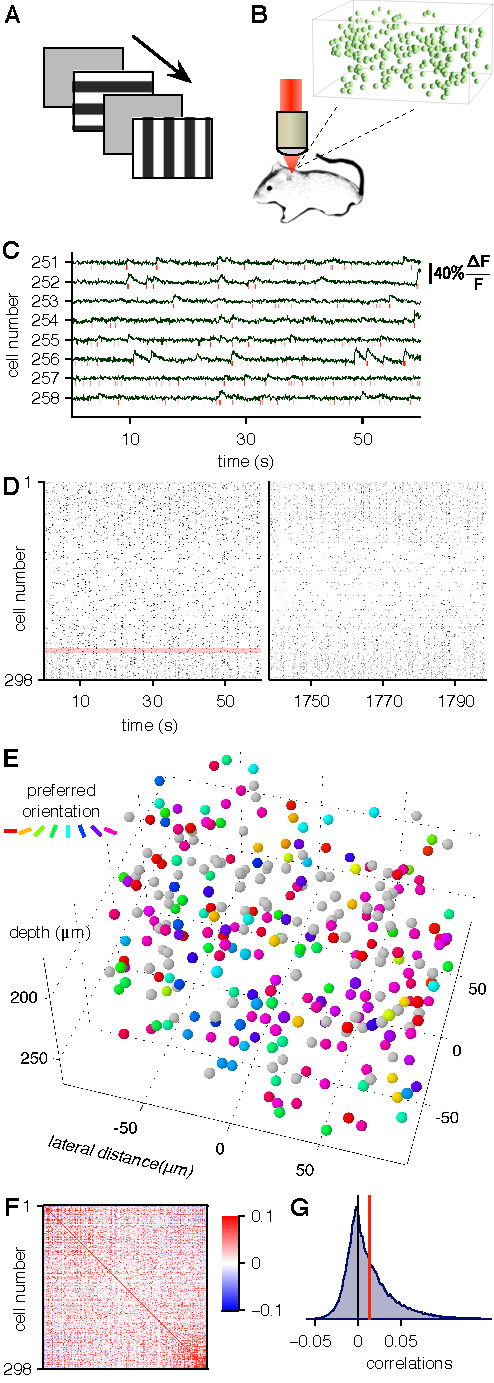
\includegraphics[width=8.3cm]{figures/Figure03.pdf}
    \end{center}
    \caption{{\bf Acquisition of neural signals for the estimation of noise correlations.}
    Visual stimuli comprising full-field drifting gratings interleaved with blank screens ({\bf A}) were presented to anesthetized mice while two-photon recordings of somatic calcium signals were collected using fast 3D random-access microscopy ({\bf B}). The visual stimulus included an initial period with 16 directions of motion for orientation tuning followed by a longer (15--20 min) period of stimulation with only 2 or 5 directions of motion for the computation of the noise correlation matrix. 
    {\bf C.} Representative calcium signals from eight cells out of 298 cells downsampled to 20 Hz. The inferred firing rate binned in 150 ms intervals are indicated by red ticks below each trace.
    {\bf D.} The raster plot of the inferred firing rates, binned in 150 ms intervals, from the entire population from the first (left) and last (right) minute of the entire recording.  The traces from {\bf C} are highlighted in red.
    {\bf E.} The spatial arrangement and orientation tuning of the 298 cells from the imaged site.
    {\bf F.} The noise correlation matrix of the activity of the neural population. 
    {\bf G.} The histogram of the noise correlation coefficients with the mean indicated by the red line.
}
    \label{fig:03}
\end{figure}

\begin{figure}[!ht]
    \begin{center}
        %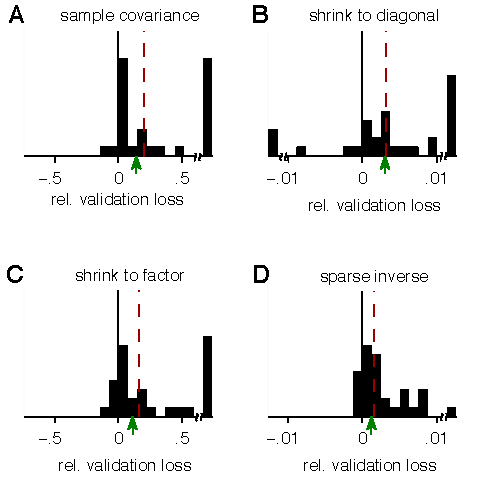
\includegraphics[width=8.3cm]{Figure04.pdf}
    \end{center}
    \caption{{\bf The sparse+latent estimator $C_{\sf sparse+latent}$ outperforms the other estimators on neural data.}
    {\bf A--D.} Histograms of average cross-validation loss differences of the respective estimators $C_{\sf 0}$, $C_{\sf diag}$, $C_{\sf factor}$, and $C_{\sf sparse}$ from $C_{\sf sparse+latent}$. 
    The histograms are based on 31 imaged sites in 24 mice. 
    All medians (red dashed lines) were significantly greater than zero, indicating the dominance of $C_{\sf sparse+latent}$ over the other estimators. 
    The green arrows indicate the results for the site shown in Fig.~\ref{fig:03} and Fig.~\ref{fig:05}
    }
    \label{fig:04}
\end{figure}
        
\begin{figure}[!ht]
    \begin{center}
        %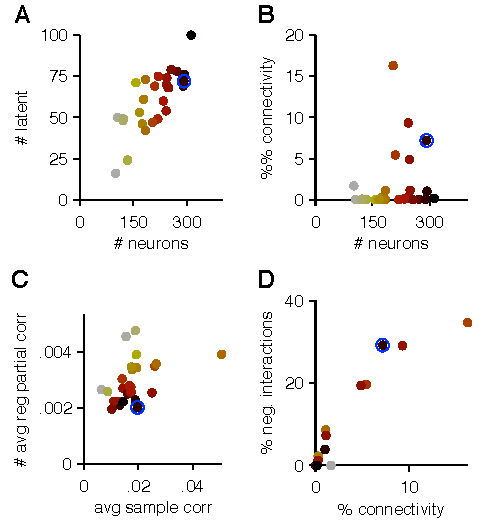
\includegraphics[width=17.35cm]{Figure05.pdf}
    \end{center}
    \caption{{\bf Example of low-dimensional correlation structure revealed by the sparse+low-rank estimator.}
    {\bf A.} The regularized estimate of the correlation matrix (top-right) closely approximates the sample correlation matrix (bottom left). 
    This close approximation is  also demonstrated by the scatter plot of the correlation coefficients produced by the two estimates ({\bf D}). 
    However, the partial correlation matrices from the two estimate show more pronounced differences ({\bf B} and {\bf E}). 
    {\bf C.} Furthermore, the partial correlation matrix of the regularized estimate is decomposed into a sparse component with 82.2\% off-diagonal zeros (bottom-left) and low-rank component of rank 15 (top-right).
    {\bf F.} The sparse component of the regularized partial correlation matrix had little resemblance to the sample correlations. The gray interval indicates the range of correlations containing 82.2\% of cells pairs, equal to the fraction of zeros in the sparse partial correlation matrix. This interval contained 58.9\% of the partial correlations. 
    {\bf G.} The graphical depiction of the positive (green) and negative (magenta) partial correlations as edges between observed neurons. The line density is proportional to the magnitude of the correlation.
    {\bf H.} A subset of neurons from the center of the cluster shown in {\bf G} showing the regularized partial correlations.
    {\bf I.} The same subset with sample correlations thresholded to match the sparsity of the regularized interactions.
}
\label{fig:05}
\end{figure}

\begin{figure}[!ht]
    \begin{center}
        %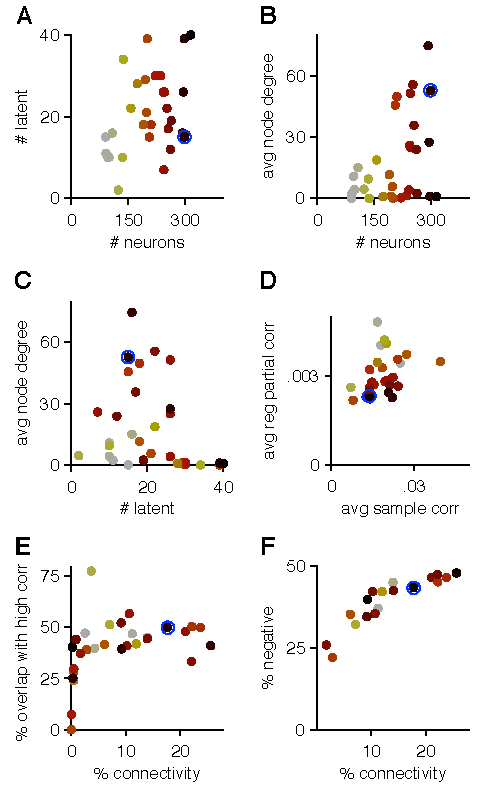
\includegraphics[width=17.35]{Figure06.pdf}
    \end{center}
    \caption{{\bf Properties of sparse+low-rank regularized estimates from all imaged sites}
    {\bf A.} The average sample correlations vs.~average partial correlations for each imaged site. In each plot, the red asterisk indicates the site shown in figures \ref{fig:03} and \ref{fig:05}.
    {\bf B.} The average node degree for sparse partial correlations vs.~population size in each imaged site. 
    {\bf C.} The number of inferred latent units vs.~population size in each imaged site.
    {\bf D.} The number latent units vs.~average node degree for sparse partial correlations for each site.
}
\label{fig:06}
\end{figure}

\begin{figure}[!ht]
    \begin{center}
        %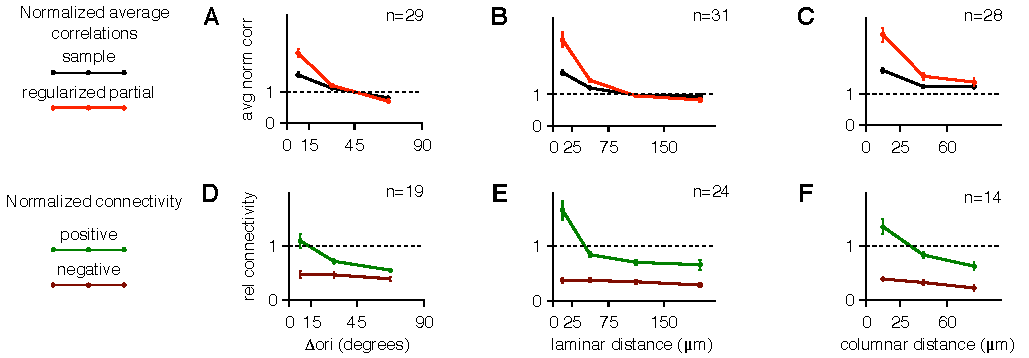
\includegraphics[width=17.35]{Figure07.pdf}
    \end{center}
    \caption{{\bf Dependence of correlations and partial correlations on orientation tuning differences and physical distance between cell pairs.}
    {\bf A--C.} Average sample correlations (black) and regularized partial correlations (red) between pairs of cells in the example site shown in previous figures. The correlations were normalized by the respective average correlations (\ref{fig:06}\,A).
    {\bf A.} Average correlations between pairs of neurons tuned to orientation with differences in preferred orientation in the intervals of 0--15$^\circ$, 15--45$^\circ$ and 45--90$^\circ$. 
    {\bf B.} Average correlations between pairs of neurons located at the same depth ($\pm$25$\mu$m) separated by lateral distances in the intervals of 0--25 $\mu$m, 25--75 $\mu$m, 75--150 $\mu$m, and 150+ $\mu$m.
    {\bf C.} Average correlations between pairs of neurons displaced laterally by less than 25 $\mu$m separated in depth by distances in the intervals of 0-25 $\mu$m, 25--60 $\mu$m, and 60+ $\mu$m.
    {\bf D--F.} Same measurements as {\bf A--D} averaged across multiple sites. Only sites that had at least 20 qualifying cell pairs in each of the intervals were included in the averages. The error bars indicate the standard error of the mean (often too small to be seen).
    {\bf G--I.} Normalized connectivity of positive (green) and negative (dark red) interactions from the sparse component of the regularized partial correlations in the example site show in previous figures. Normalized connectivity was computed as the fraction of pairs connected by interactions of corresponding signs in each interval divided by fraction of non-zero interactions across the entire site. The intervals are identical to those in {\bf A--C}.
    {\bf J--L.} Same measurements as in {\bf G--I} averaged across multiple sites. The error bars indicate the error of the mean. Only sites that had at least 20 qualifying pairs in each interval were included in the averages. 
}
\label{fig:07}
\end{figure}

\end{document}
